\section{Two-dimensional systems and their vector fields}
\label{sec:twodimaut}

\LAtt{3.5}

\LO{
\item Visualize and sketch the behavior of a two dimensional system based on the eigenvalues and eigenvectors.
}


In the last three sections, we looked at the different options for two-component constant-coefficient systems. We want to determine a nice way to put all of this together. We summarize the behavior of linear homogeneous two-dimensional systems
given by a nonsingular matrix
in \tableref{pln:behtab}.
Systems where one of the eigenvalues is zero (the matrix is singular)
come up in practice from time to time, see
\examplevref{sintro:closedbrine-example}, and the pictures are somewhat
different (simpler in a way).  See the exercises.

\begin{table}[h!t]
\mybeginframe
\capstart
\begin{center}
\begin{tabular}{@{}ll@{}}
\toprule
Eigenvalues & Behavior \\
\midrule
real and both positive & source / unstable node \\
real and both negative & sink / asymptotically stable node \\
real and opposite signs & saddle \\
purely imaginary & center point / ellipses \\
complex with positive real part & spiral source \\
complex with negative real part & spiral sink \\
repeated with two eigenvectors & proper node  (asympt. stable or unstable) \\
repeated with one eigenvector & improper node (asympt. stable or unstable) \\
\bottomrule
\end{tabular}
\end{center}
\caption{Summary of behavior of linear homogeneous two-dimensional systems.\label{pln:behtab}}
\myendframe
\end{table}

The sketches of all of these different behaviors and phase portraits can be found in their respective sections. Make sure that you understand the terminology, general behavior, and sketches for each of these different cases. 

\subsection{Trace-Determinant Analysis}

One other way to interpret and analyze this information is using the trace and determinant of the matrix. Recall from \sectionref{sec:kernel} that the \myindex{trace} of a matrix is the sum of the diagonal entries of the matrix and the \myindex{determinant} of the matrix is computed from the entries and is a way to determine invertibility of the matrix. If we take a generic $2 \times 2$ matrix and find the characteristic polynomial, we get that for
\begin{equation*}
A = \begin{bmatrix} a & b \\ c & d \end{bmatrix},
\end{equation*}
the characteristic polynomial is 
\begin{equation*}
\det(A - \lambda I) = (a - \lambda)(d - \lambda) - (b)(c) = \lambda^2 - (a+d)\lambda + (ad-bc).
\end{equation*}
Since the trace of the matrix is $a+d$ and the determinant is $ad-bc$, we can rewrite this polynomial as
\begin{equation*}
\lambda^2 - T\lambda + D = 0,
\end{equation*}
which also means that we can characterize the eigenvalues of the matrix in terms of the trace and determinant. We get that the eigenvalues are
\begin{equation}
\lambda = \frac{T \pm \sqrt{T^2 - 4D}}{2}.
\label{eq:eigenTD}
\end{equation}

There are a few important facts we can learn from this equation. 
\begin{enumerate}[1.]
\item A lot depends on the value of $T^2 - 4D$. If $T^2 - 4D > 0,$ then we will have two real distinct eigenvalues. If $T^2 - 4D = 0,$ then there is a single repeated eigenvalue, and if $T^2 - 4D < 0$, we have complex eigenvalues.
\item If $D < 0$, then $T^2 - 4D > T^2,$ which means that $\sqrt{T^2 - 4D} > |T|$. If we put this into \eqref{eq:eigenTD}, this will mean that the term that is after the $\pm$ will be larger than $T$ in absolute value. Therefore, the two eigenvalues will be real and have opposite signs.
\item If $D \geq 0$, then the sign of the eigenvalues, or the sign of the real part in the complex case, is dictated by the sign of $T$. If $D \geq 0$, then $T^2 - 4D \leq T^2$, so that the part under the square root in \eqref{eq:eigenTD} is always smaller in absolute value than $T$. Thus, both the plus and minus version will have values that are the same sign as $T$. If the expression is complex, then the real part is exactly $T/2$, which is the same sign as $T$. 
\end{enumerate}

All of this means we can make a new table characterizing the eigenvalues and how they are connected to the trace and determinant. 

\begin{table}[h!t]
\mybeginframe
\capstart
\begin{center}
\begin{tabular}{@{}ll@{}}
\toprule
Eigenvalues & Trace and Determinant Classification \\
\midrule
real and both positive & $T > 0$, $D > 0$, $T^2 - 4D > 0$  \\
real and both negative &  $T < 0$, $D > 0$, $T^2 - 4D > 0$\\
real and opposite signs & $D < 0$ \\
purely imaginary &  $T = 0$, $D > 0$\\
complex with positive real part & $T > 0$, $T^2 - 4D < 0$  \\
complex with negative real part &  $T < 0$, $T^2 - 4D < 0$ \\
repeated & $T^2 - 4D = 0$ \\
\bottomrule
\end{tabular}
\end{center}
\caption{Summary of behavior of linear homogeneous two-dimensional systems.\label{pln:behtabTD}}
\myendframe
\end{table}

Since these are all based on the relation between $T$ and $D$, we can also combine all of this into a figure to summarize the details. In \figurevref{fig:TDPlaneAnalysis}, $T$ is on the horizontal axis and $D$ is the vertical axis. The graph drawn is $D = \nicefrac{T^2}{4}$, which is the important criteria that shows up in the table. 

\begin{myfig}
\capstart
\myincludegraphics{width=5.5in}{width=5in}{eigTraceDet}
\caption{Trace-Determinant plane for analysis of two-component linear systems. \label{fig:TDPlaneAnalysis}}
\end{myfig}

\figurevref{fig:TDPlaneAnalysis} can be used to determine the behavior of a two-component system without actually needing to solve the differential equation. The point is that the signs and type of the eigenvalues determine the structure of the solution, and we can determine the important qualities of these using just the trace and determinant of a matrix.

\begin{example}
Use Trace-Determinant analysis to determine the overall behavior of the system
\begin{equation*}
{\vec{x}}' = \begin{bmatrix} 1 & 4 \\ -2 & 3 \end{bmatrix}\vec{x}.
\end{equation*}
\end{example}

\begin{exampleSol}
From the matrix, we can see that the trace is $1 + 3  = 4$ and the determinant is $(1)(3) - (4)(-2) = 11$. We see that $D > 0$ with $T^2 = 16$ and $4D = 44 > 16$. Therefore, we have $4D > T^2$, so we are above the curve on the graph, and so have a spiral. Since $T > 0$, this will be a spiral source. 

\textbf{Note:} If you wanted to get a general solution or sketch a phase portrait for this differential equation, you would need to actually solve it out for that; you can not get enough information just from this image to sketch a proper phase portrait.
\end{exampleSol}

\begin{exercise}
Compute the eigenvalues for the system above, find the general solution, and verify that this is a spiral source. The numbers here will not work out great, so having the quick analysis that it is a spiral source is nice. 
\end{exercise} 
 

\subsection{Exercises}

\begin{exercise}
Take the equation $m x'' + c x' + kx = 0$, with $m > 0$, $c \geq 0$, $k > 0$
for the mass-spring system.
\begin{tasks}
\task Convert this to a system of first
order equations.
\task Classify for what $m, c, k$ do you get which behavior.
\task Can you explain from physical intuition why you do not get all the
different kinds of behavior here?
\end{tasks}
\end{exercise}
\comboSol{%
}
{%
a)~${\vec{x}}' = \left[\begin{smallmatrix} 0 & 1 \\ -k/m &-c/m \end{smallmatrix}\right]\vec{x}$ \quad b)~$c=0$ is center, $c^2 - 4mk < 0$ is spiral sink, $c^2 - 4mk = 0$ is improper sink, $c^2 - 4mk > 0$ is nodal sink. \quad c)~The forced positive coefficients restricts the behavior 
}

\begin{exercise}
What happens in the case when $P = 
\left[ \begin{smallmatrix} 1 & 1 \\ 0 & 1 \end{smallmatrix} \right]$?  In
this case the eigenvalue is repeated and there is only one independent eigenvector.
What
picture does this look like?
\end{exercise}
\comboSol{%
}
{%
Improper nodal sink \hfill\raisebox{-0.5\height}{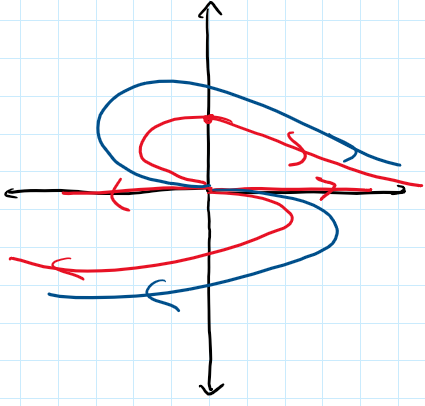
\includegraphics[height=1.5in]{Images/phaseportrait_1_1_0_1_sketch.png}}\hfill\hfill
}

\begin{exercise}
What happens in the case when $P = 
\left[ \begin{smallmatrix} 1 & 1 \\ 1 & 1 \end{smallmatrix} \right]$?
Does this look like any of the pictures we have drawn?
\end{exercise}
\comboSol{%
}
{%
It does not look like any of our previous pictures. \hfill\raisebox{-0.5\height}{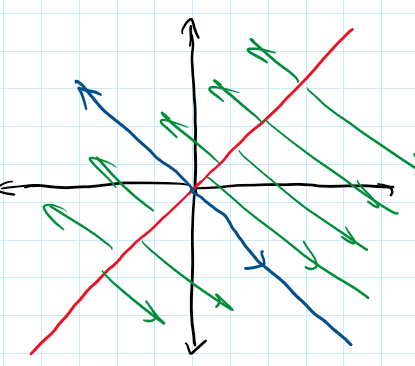
\includegraphics[height=1.5in]{Images/phaseportrait_1_1_1_1_sketch.png}}\hfill\hfill
}

\begin{exercise}\ansMark%
Describe the behavior of the following systems without solving:
\begin{tasks}(2)
\task $x' = x + y$, \quad $y' = x-y$.
\task $x_1' = x_1 + x_2$, \quad $x_2' = 2 x_2$.
\task $x_1' = -2x_2$, \quad $x_2' = 2 x_1$.
\task $x' = x + 3y$, \quad $y' = -2x-4y$.
\task $x' = x - 4y$, \quad $y' = -4x+y$.
\end{tasks}
\end{exercise}
\exsol{%
a) Two eigenvalues: $\pm \sqrt{2}$ so the behavior is a saddle.
\quad
b) Two eigenvalues: $1$ and $2$, so the behavior is a source.
\quad
c) Two eigenvalues: $\pm 2i$, so the behavior is a center (ellipses).
\quad
d) Two eigenvalues: $-1$ and $-2$, so the behavior is a sink.
\quad
e) Two eigenvalues: $5$ and $-3$, so the behavior is a saddle.
}

\begin{exercise}
Which behaviors are possible if $P$ is diagonal, that is
$P = \left[ \begin{smallmatrix} a & 0 \\ 0 & b \end{smallmatrix} \right]$?
You can assume that $a$ and $b$ are not zero.
\end{exercise}
\comboSol{%
}
{%
Eigenvalues are $a$ and $b$, so any real eigenvalue behavior is possible. Saddle, source, sink.
}

\begin{exercise}\ansMark%
Suppose that $\vec{x}\,' = A \vec{x}$ where $A$ is a 2 by 2 matrix
with eigenvalues $2\pm i$.  Describe the behavior.
\end{exercise}
\exsol{%
Spiral source.
}

\begin{exercise}\ansMark\label{ex:TwoDimSys1}%
For each of the following matrices $A$, describe the behavior and classify the phase portrait of the system given by ${\vec{x}}' = A\vec{x}$. Use the eigenvalues to determine this.
\begin{tasks}(2)
\task $A = \begin{bmatrix} 7 & -8 \\ 3 & -3 \end{bmatrix}$
\task $A = \begin{bmatrix} 3 & 5 \\ -1 & 1 \end{bmatrix}$
\task $A = \begin{bmatrix} 8 & -18 \\ 4 & -10 \end{bmatrix}$
\task $A = \begin{bmatrix} -2 & -4 \\0 & -3 \end{bmatrix}$
\task $A = \begin{bmatrix} 3 & -2 \\ 2 & -3 \end{bmatrix}$
\task $A = \begin{bmatrix} -3 & -4 \\ 1 & 1 \end{bmatrix}$
\end{tasks}
\end{exercise}
\exsol{%
a) Nodal source \quad c) Spiral source  \quad  c) Saddle \quad c) Nodal sink \quad  e) Spiral sink \quad f) Improper nodal sink
}

\begin{exercise}
For each of the matrices and systems in \exerciseref{ex:TwoDimSys1}, perform the same analysis using the trace and determinant of the matrix.
\end{exercise}

\begin{exercise}
Consider the system of differential equations given by 
\begin{equation*}
{\vec{x}}'  = \begin{bmatrix} -2 & -3 \\ 3 & -2 \end{bmatrix} \vec{x}.
\end{equation*}
\begin{tasks}
\task Use trace and determinant analysis to determine the behavior of this linear system.
\task Find the general solution to this system of differential equations and verify that it matches the analysis in (a).
\end{tasks}
\end{exercise}
\comboSol{%
}
{%
Spiral sink. $\vec{x}(t) = C_1e^{-2t}\left[\begin{smallmatrix} -\sin(3t) \\ \cos(3t) \end{smallmatrix}\right] + C_2e^{-2t} \left[\begin{smallmatrix} \cos(3t) \\ \sin(3t) \end{smallmatrix}\right]$.
}

\begin{exercise}
Consider the system of differential equations given by 
\begin{equation*}
{\vec{x}}'  = \begin{bmatrix} -2 & -3 \\ 3 & 4 \end{bmatrix} \vec{x}.
\end{equation*}
\begin{tasks}
\task Use trace and determinant analysis to determine the behavior of this linear system.
\task Find the general solution to this system of differential equations and verify that it matches the analysis in (a).
\end{tasks}
\end{exercise}
\comboSol{%
}
{%
Improper nodal source. $\vec{x}(t) = C_1 \left[\begin{smallmatrix} 1 \\ -1 \end{smallmatrix}\right]e^t + C_2\left(\left[\begin{smallmatrix} 1 \\ -1 \end{smallmatrix}\right]te^t + \left[\begin{smallmatrix} -1/3 \\ 0 \end{smallmatrix}\right]e^t \right)$
}

\begin{exercise}
Take the system from \examplevref{sintro:closedbrine-example},
$x_1'=\frac{r}{V}(x_2-x_1)$,
$x_2'=\frac{r}{V}(x_1-x_2)$.
As we said, one of the eigenvalues is zero.  What is the other eigenvalue, how
does the picture look like and what happens when $t$ goes to infinity.
\end{exercise}
\comboSol{%
}
{%
All solutions flow directly to the line $y=x$.
}

\begin{exercise}\ansMark%
Take
$\left[ \begin{smallmatrix}
x \\ y
\end{smallmatrix}\right] '
=
\left[ \begin{smallmatrix}
0 & 1 \\ 0 & 0
\end{smallmatrix}\right]
\left[ \begin{smallmatrix}
x \\ y
\end{smallmatrix}\right]$.
Draw the vector field and describe the behavior.  Is it one of the
behaviors that we have seen before?
\end{exercise}
\exsol{%
\\[6pt]
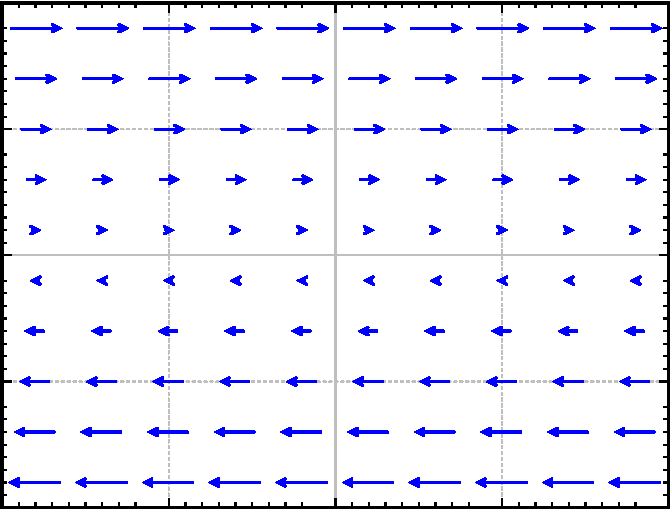
\includegraphics[width=2in]{figures/0100vectorfield}
\\
The solution does not move anywhere if $y = 0$.  When $y$ is positive,
the solution moves (with constant speed)
in the positive $x$ direction.  When $y$ is
negative, the solution moves (with constant speed) in the negative
$x$ direction.  It is not one of the behaviors we have seen.
\\
Note that the matrix has a double eigenvalue 0 and the general solution is
$x = C_1 t + C_2$ and $y = C_1$, which agrees with the
description above.
}

\begin{exercise}
In this exercise, we will analyze ``perturbations'' or near-by matrices to the ones that are given. This will be important later in \sectionref{linearization:section}. For each of the following matrices
\begin{tasks}
\task Find the trace and determinant, and use them to classify the behavior of the linear system ${\vec{x}}' = A\vec{x}$ for the given matrix $A$.
\task Draw a sketch of the trace-determinant plane, including the curve $D = \nicefrac{T^2}{4}$, and plot the point corresponding to the matrix on those axes.
\task Look at the points in a small (as small as you want) circle around the point you just drew. What does the behavior look like for systems whose matrices fall within that circle? What do these behaviors have in common with each other, and how do they differ?
\end{tasks}
\begin{equation*}
\begin{split}
(i)\ \begin{bmatrix} 2 & 8 \\ -3 & -8 \end{bmatrix} \qquad (ii)\ \begin{bmatrix} 15 & -12 \\ 16 & -13 \end{bmatrix} \qquad &(iii)\ \begin{bmatrix} 2 & -1 \\ 5 & -2 \end{bmatrix} \qquad (iv)\ \begin{bmatrix} 4 & -1 \\ 2 & 2 \end{bmatrix}\\
(v)\ \begin{bmatrix} -2 & 2 \\ -2 & -6 \end{bmatrix} \qquad (vi)\ \begin{bmatrix} -1 & -4 \\ 2 & 5 \end{bmatrix} \qquad &(vii)\ \begin{bmatrix} -5 & 6 \\ -3 & 1 \end{bmatrix} \qquad (viii)\ \begin{bmatrix} 5 & -2 \\ 8 & -3 \end{bmatrix} 
\end{split}
\end{equation*}
\end{exercise}
\exsol{%
(i) $T=-6$, $D = 8$. Nodal sink. All points nearby are nodal sinks. \\
(ii)  $T = 2$, $D = -3$. Saddle. All points nearby are saddles. \\
(iii)  $T = 0$, $D = 1$. Center. Points nearby are all spirals, but they could be asymptotically stable, centers, or unstable. Stability is unknown.\\
(iv)  $T = 6$, $D = 10$. Spiral source. All points nearby are spiral sources.\\
(v)  $T = -8$, $D = 16$. Improper nodal sink. All points nearby will be asymptotically stable, but they could be nodal sinks, improper nodal sinks, or spiral sinks.\\
(vi)  $T = 4$, $D = 3$. Nodal source. All points nearby are nodal sources. \\
(vii)  $T = -4$, $D = 13$. Spiral sink. All points nearby are spiral sinks. \\
(viii)  $T = 2$, $D = 1$. Improper nodal source. All points nearby will be unstable, but they may be spirals, nodal sources, or improper nodal sources.\\
}%


\setcounter{exercise}{100}
